\documentclass[11pt,a4paper,oneside]{article}
\usepackage{amsmath,amsthm,amssymb,amsfonts,adjustbox,bm}
\usepackage{geometry}
\usepackage{threeparttable}
\geometry{margin=1.2in}
%\usepackage[dvipsnames]{xcolor}
\usepackage{mathtools}
\usepackage{refstyle}
\usepackage{pdflscape}
\usepackage{longtable}
\usepackage{eurosym}
\usepackage{enumerate}
\usepackage{booktabs}
\usepackage{siunitx}
\usepackage{rotating}
\usepackage{graphicx}
\usepackage{subcaption}
\usepackage{caption}
\usepackage[section]{placeins}
\usepackage{xcolor}
\usepackage{geometry}
\usepackage{changepage}
\usepackage[natbibapa]{apacite}
\usepackage{threeparttable}
\newcommand{\footremember}[2]{%
   \footnote{#2}
    \newcounter{#1}
    \setcounter{#1}{\value{footnote}}%
}
\newcommand{\footrecall}[1]{%
    \footnotemark[\value{#1}]%
} 


\usepackage[colorlinks=true, citecolor=blue, linkcolor=blue, urlcolor=blue,breaklinks]{hyperref}


% \title{Skills, Inequality, and Referrals \\ \large Experimental Design \\}
\title{Skills, Inequality, and Referrals}
\author{Jhon Díaz\footnote{Universidad Autónoma de Bucaramanga}, Manuel Munoz\footremember{liser}{Luxembourg Institute of Socio-Economic Research}, Ernesto Reuben\footnote{Division of Social Science, New York University Abu Dhabi} \footrecall{liser}, Reha Tuncer\footnote{University of Luxembourg}}
% \footnote{Center for Behavioral Institutional Design at New York University Abu Dhabi} 
\begin{document}

\maketitle



\section*{Abstract}

Through the sharing of opportunities from wealthier and educated individuals, ties across socioeconomic backgrounds lead to better outcomes (i.e., upward mobility). 
Referrals propagate inequality because they tend to be similar across many observable dimensions, making them problematic for diversity. Yet, ties across socioeconomic backgrounds to wealthier and educated individuals lead to better outcomes (i.e., upward mobility) through the sharing of opportunities. For ties to form, though, simple exposure is not enough: Individuals across social classes should befriend each other to benefit. Universities are potentially one such environment where exposure and friendship among different social classes are plenty. Can quotas change referral choices? And if so, do different skill requirements lead to particular referrals? We conduct an incentivized field experiment in a Colombian university to measure the effects of (i) a low social class quota and (ii) two different skill requirements on referral composition and quality. \medskip \\
\textbf{JEL Classification:} \\
\textbf{Keywords:} behavioral economics, referrals, field experiment, skills, inequality, upward mobility

\section{Introduction}

Socioeconomic background significantly influences life outcomes, with individuals from lower socioeconomic status (SES) typically having fewer professional opportunities and lower lifetime earnings. Chetty et al. (2022) show that low-SES individuals with ties to high-SES individuals achieve significantly better earnings, underscoring social networks as a potential mechanism for upward income mobility. The fundamental hypothesis is that once a tie is formed, information and opportunities flow from high-SES connections to low-SES individuals, by shaping aspirations or by providing job referrals.

For ties to form, high-SES and low-SES individuals need to share common spaces. Universities, among a few other settings, are diverse enough for interactions across social groups to take place. As individuals from different social classes interact throughout college, the availability issue disappears. Yet, it is unclear whether having the opportunity to form ties is sufficient for beneficial flows to occur. Social groups exhibit significant homophily across observable characteristics, which may restrict these beneficial flows inside networks. To address this gap, we investigate the extent of information and opportunity transfers from high-SES to low-SES students in a university setting. We seek to answer two research questions: To what extent do high-SES students provide referrals to low-SES classmates in college? Can a quota system incentivize students to refer equally qualified low-SES peers, thereby reducing inequalities in referrals?

We conducted a lab-in-the-field experiment at our partner university in Colombia, involving 693 students. We collected objective skill measures and asked participants to make referrals among their classmates. Referrers were incentivized based on performance. We also included an incentivized social class guessing task and restricted network choice sets to the classroom, allowing us to collect skill measures for all potential referrals and referrers and to fix SES compositions at the classroom level. We exploited Colombia's unique administrative feature where state-assigned SES levels are common knowledge. This setup allowed for clean identification of the SES-relationship between referrals and referrers, controlling for performance, SES composition, and the ability to identify social class.

Early findings indicate that referrals are concentrated at the SES level, with high-SES individuals referring other high-SES at a significantly higher rate compared to their sample share. Low-SES constitute around 60% of the sample and refer to other low-SES at a similar rate, resulting in no general bias against low-SES. Above-median scores across two objective skill measures suggest high-SES preference to refer other high-SES is not driven by performance concerns.

Our second research question focused on whether a quota system could alleviate referral inequalities. Half of our sample was assigned to a quota treatment incentivizing referrals of high-performing low-SES individuals, but this did not cause a statistically significant shift in low-SES referrals. Classroom SES compositions reveal low-SES referrals to be mainly driven by availability for both low- and high-SES referrers.

In conclusion, the presence of low-SES individuals in college appears sufficient to ensure that cross-SES interactions translate into tangible benefits for disadvantaged groups, primarily through increased availability in referral networks rather than changes in referral behavior.


\section{Background and Empirical Setting}

\subsection{Related Literature}

\subsection{Socioeconomic background in Colombia}

\section{Design}
\subsection*{Overview}
Our study design comprises an experiment with three sequential parts (see Figure \ref{timeline}). We conducted all parts of the experiment, including the demographic survey, in April 2024. In the first part, participants complete incentivized skill tests, and we elicit their beliefs about their performance. The second part involves participants referring classmates for each of the skill tests. The third and final part consists of a socioeconomic background (SEB) guessing task. We provide the complete experimental instructions in Appendix \ref{instructions}.

\begin{figure}[htbp]
  \centering
  \includegraphics[scale=0.09]{timeline.jpg}
  \caption{Participants went through the study design in the order presented here.}\label{timeline}
\end{figure}

\subsection{Skill Assessment}\label{skill_assessment}

This part consists of two incentivized skill tests. The tests are presented in a randomized order and participants are asked to answer the items to the best of their ability. There is a 5-minute timer for each test due to time constraints and no performance feedback is provided at any time. Participants read the test-specific instructions first and go through an example item before beginning each test. During the tests, participants are not forced to answer items and can skip them if they choose to do so. Participants see one item at a time and cannot return to previous screens once they start a test.\footnote{After each test, we also elicited beliefs about participants' performance. These beliefs are not directly related to our theoretical framework and were not incentivized.} \medskip\\
\textbf{Cognitive Skills.} We use Raven's Progressive Matrices to measure cognitive skills \citep{raven_performances_1936, raven_standard_1976}. Raven’s test is a well-established measure of fluid intelligence, i.e., an individual’s capacity to reason and solve problems in novel situations independent of past knowledge \citep{schilbach_psychological_2016}. In this test, participants see series of images where there is a pattern with a piece that has been intentionally removed. They are tasked with choosing the piece that completes the pattern among available options. For each image, there is only one correct answer. We implement an 18-item version featuring increasingly difficult questions, with 6 response options for the first 9 items and 8 thereafter.  \medskip\\
\textbf{Social Skills.} We measure social skills with the Multiracial Reading the Mind in the Eyes Test (MRMET) from \citet{kim_multiracial_2022}. Based on the original RMET \citep{baron-cohen_reading_2001}, the MRMET is a race- and gender-inclusive test suitable for application in non-WEIRD (Western, Educated, Industrial, Rich, Democratic) populations that measures the ability to recognize emotions in others. The test has been previously used in economic experiments \citep{van_leeuwen_predictably_2018, weidmann_team_2021}. MRMET consists of photos of human faces portraying different emotions, cropped so that only the eye region is visible. Participants must choose the emotion that best describes the photo from the available answers (see the example in Figure \ref{emotions-example}). For each photo, there is only one correct answer and 4 response options. We administer the first 36 items in MRMET.  \medskip\\
\textbf{Incentives.} 20\% of participants in each classroom are randomly selected to be eligible for a bonus worth 100,000 Pesos (about \$26 in April 2024) for this part. A computer algorithm randomly selects one skill test for each eligible participant and draws a number between 1 and 100. The participant receives the bonus if the percentage of correct answers in the selected test exceeds that number. Conditional on the skill test being selected (1/2), chances to earn the bonus increase with each correctly solved question by 5.5\% (=1/18) for the Cognitive Skills test and by 2.78\% (=1/36) for the Social Skills test.


\begin{figure}[htbp]
  \centering
  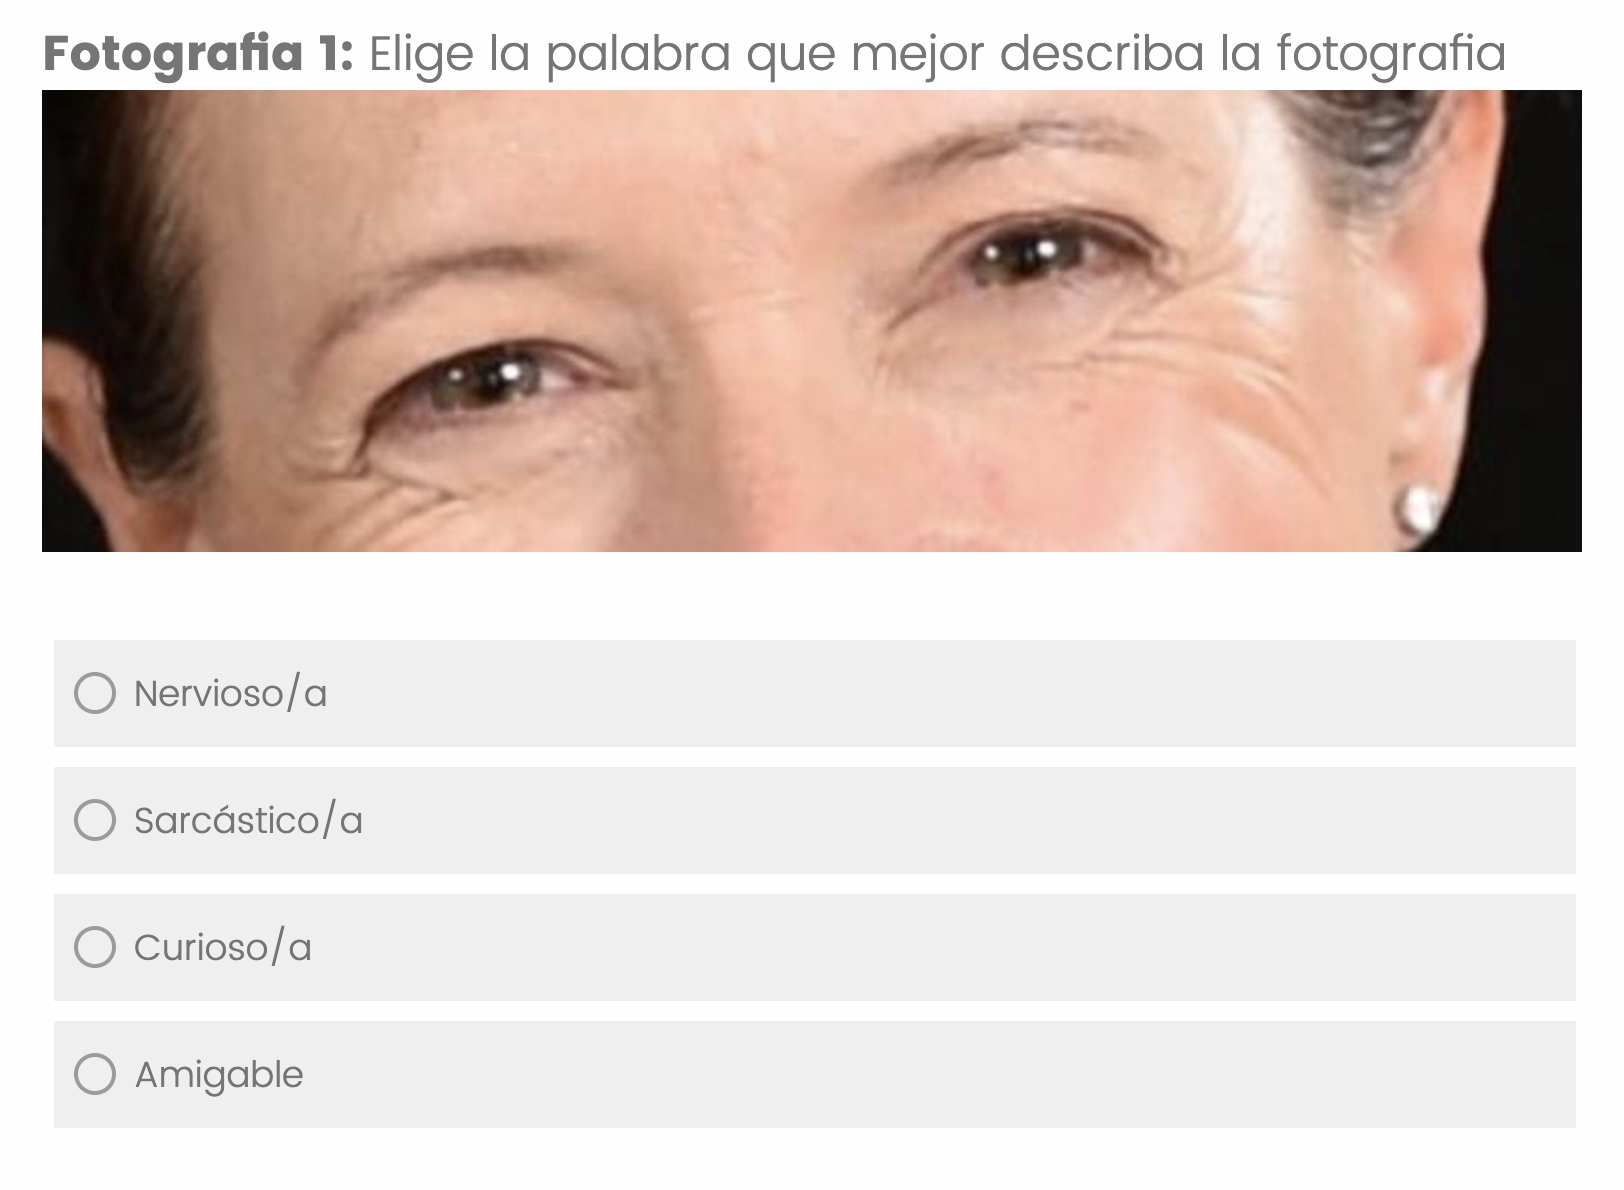
\includegraphics[scale=0.3]{social-skill-example.png}
  \captionsetup{width=0.8\linewidth}
  \caption{Example item from the Multiracial Reading the Mind in the Eyes Test (MRMET). The correct answer for this item (translated from Spanish ``Amigable") is Friendly.}\label{emotions-example}
\end{figure}

\subsection{Referral Task} \label{referral_task}
In part two, participants make referrals by nominating people they believe scored the highest on the skill tests. The order in which they refer for a given skill test is randomized. For each test, participants receive an explanation of what skill was measured accompanied by an example item, before making referrals. On the following page, participants see an alphabetically ordered list of all individuals in their classroom by first names. Providing this list instead of an empty free text field could help alleviate biases related to recall in referral choice. Participants are asked to make three referrals per skill. They are instructed to exclude themselves from referrals, even though their names are on the list. This self-exclusion serves as an attention check. A classmate may be nominated once per triad and referring the same individual twice is only possible when nominated for both skills. There are no timers in this part, but the decision time is recorded. \medskip\\
\textbf{Top 3.} We establish classroom-level rankings to incentivize referrals based on performance. Within each classroom, participants are ranked according to the number of correct answers they provide for a particular skill test. The three highest-scoring classmates are designated as the top 3 for that specific skill in their classroom. In instances where there is a tie for any position among the top 3, a computer algorithm randomly determines the final top 3 participants. This ranking system serves as the foundation for assessing the accuracy of participant referrals within each classroom context.\medskip\\
\textbf{Incentives.} We offer incentives for referrals of the top 3 performers for each skill within each classroom. 40\% of participants in each classroom are randomly selected to be eligible for a bonus worth 100,000 Pesos (about \$26). A computer algorithm randomly selects one skill test and one referral for each eligible participant. The participant receives the bonus if their selected referral is among the top 3 for that specific skill.\medskip\\
\textbf{Treatment.} The experiment comprises two treatment conditions, with the selection procedure for the top 3 in the referral task as the variable of interest. In the \textbf{Baseline} condition, the top 3 selection is based solely on test performance, regardless of other participant characteristics. Participants are ranked according to the number of correct answers they provide for a particular skill test in each classroom. The \textbf{Quota} condition modifies the top 3 selection to prioritize lower-SEB individuals. Here, the first spot in the top 3 for both skills is reserved for the highest-scoring lower-SEB classmate, with the remaining two places assigned based on test performance. This guarantees at least one lower-SEB participant in the top 3 per skill. Participants are informed about the top 3 selection mechanism before making referrals and the incentive structure remains unchanged: Referrals among the top 3 are always eligible for the 100,000 Pesos bonus. Assignment to the treatment conditions is at the individual level within each classroom, allowing a comparison of the top 3 selection mechanism while keeping the referral choice set constant.

\subsection{SEB Guessing Task}\label{guessing_task}
In part three, participants make guesses about the anticipated SEB of their classmates. Task instructions are designed to minimize potential stigma related to SEB. Participants are informed that a computer algorithm will randomly select three students belonging to strata 1, 2, or 3, which characterize the lower-SEB in Colombia. Participants are tasked with nominating the three people they believe the computer would choose at random. They select three classmates from an alphabetically ordered list by first names containing all individuals in their classroom. This task measures the ability to distinguish SEB independent of test performance, as SEB identification is central to our study. The choice set for this task includes the participant themselves due to the specific instructions for this part. There are no time limits, but the decision time is recorded. \medskip\\ 
\textbf{Incentives.} We offer incentives for correct identification of lower-SEB individuals within each classroom. 20\% of participants in each classroom are randomly selected to be eligible for a bonus worth 100,000 Pesos (about \$26). A computer algorithm randomly selects one guess for each eligible participant. The participant receives the bonus if the selected guess correctly identifies a lower-SEB classmate.
\section{Sample and Procedure}
\textbf{Sample.} We conducted the experiment at Universidad Autónoma de Bucaramanga (UNAB), a private Colombian university with approximately 10,000 students. We invited 863 undergraduate students from 35 classrooms to participate in the experiment, representing the maximum achievable sample size. To mitigate potential selection bias related SEB, all invited students were enrolled in courses that combine multiple academic programs.\footnote{Previous studies at this university have shown that students from higher socioeconomic backgrounds tend to select finance and business administration programs, while those from lower socioeconomic backgrounds often choose STEM.} The average classroom size was 25 students. Our final sample consisted of 713 individuals who completed the study protocol, resulting in an 83\% participation rate. Table \ref{tab:my-table} presents key demographic characteristics and academic performance indicators across treatment conditions. The sample is well-balanced between the Baseline (n = 368) and Quota (n = 334) conditions. We observe no statistically significant differences in any of the reported variables (all \textit{p} $> .1$), indicating successful randomization into treatment conditions. The sample is characterized majoritarily of lower-SEB students (57\%), with about one-third of the sample (35\%) being first-generation college students. The gender distribution is balanced, with 50\% female participants. The mean GPA of 3.95 is consistent across both treatment conditions.

\begin{table}[htbp]
\centering
\begin{threeparttable}
\caption{Comparison of demographic characteristics and GPA across treatment conditions}
\begin{tabular*}{0.8\textwidth}{@{\extracolsep{\fill}}lccc c@{}}
\toprule
 & \multicolumn{1}{c}{\textbf{Sample}} & \multicolumn{1}{c}{\textbf{Baseline}} & \multicolumn{1}{c}{\textbf{Quota}} & \multicolumn{1}{c}{\textit{\textbf{p}}} \\ \midrule
Lower-SEB & .57 & .59 & .55 & \multicolumn{1}{c}{.297} \\
First Generation & .35 & .34 & .37 & \multicolumn{1}{c}{.386} \\
Female & .50 & .52 & .47 & \multicolumn{1}{c}{.195} \\
GPA & 3.95 & 3.95 & 3.95 & \multicolumn{1}{c}{.828} \\
\bottomrule
\end{tabular*}
\begin{tablenotes}[flushleft]
\footnotesize
\item[] \textit{Note:} Lower-SEB, First Generation, and Female represent binary outcomes and \textit{p}-values for these variables are from two-sample tests of proportions. For GPA, \textit{p}-value is from a two-sample t-test with unequal variances. All reported \textit{p}-values are two-tailed. 11 additional participants completed the skill tests without being assigned to a treatment condition.
\end{tablenotes}
\label{tab:my-table}
\end{threeparttable}
\end{table}


\noindent \textbf{Procedure.} Data collection occurred during the last week of April 2024. Our local partner, the Social Bee Lab at UNAB, coordinated scheduled classroom visits and recruited research assistants to administer the study protocol. Students present in class on the scheduled visit dates participated in the experiment. Each classroom visit constituted a separate data collection session. Participants accessed the Qualtrics-based experiment using their smartphones during these visits. The median time to complete the survey was 20 minutes, with an average compensation of \$4.3 per participant. After visiting all 35 classrooms, we sent private invitations to students who were absent during the scheduled sessions. These students received the survey link via their student email and had an additional week to participate. We obtained Institutional Review Board approvals from NYU Abu Dhabi (HRPP 2024-50) and the University of Luxembourg (ERP 24–028). The study design was preregistered and archived in the OSF Registries prior to data collection (see \url{https://doi.org/10.17605/OSF.IO/V9T3W}).

% \section{Variables}

% \subsection{General Description}
% The study begins with a demographic survey. The rest of the study is divided into three parts. Participants perform various experimental tasks designed to obtain behavioral measures in each part. Participants’ choices in these tasks are incentivized and determine their bonus earnings. In addition to the demographic survey and behavioral measures, UNAB provides complementary administrative data.

% \subsection{Demographic Survey Questions}
% \textbf{Gender.} We ask participants: ``What is your gender?" Answer options: Man, Woman.\medskip \\
% \textbf{Stratum.} We ask participants: ``What is the socio-economic stratum to which your family belongs?" Answer options range from 1 to 6. This is a government-assigned number assigned to every household in Colombia based on neighborhood-level wealth. It's a widely recognized classification system that directly affects utility costs and is visible on all utility bills. It categorizes neighborhoods into six strata, from 1 (lowest socioeconomic status) to 6 (highest socioeconomic status). Residents in higher strata pay more for utilities, while those in lower strata receive subsidies.\medskip \\
% \textbf{Parental Education.} We ask participants: ``What is the highest level of education acquired by your father (mother)?" Answer options are: Primary school, High school, Technical school, Undergraduate, Graduate, Postgraduate, Not applicable.

% \subsection{Administrative Data}
% \textbf{Co-enrollment History.} UNAB provides the co-enrollment history of participants in this study. This is a detailed list of all the classes participants have taken since their enrollment at the university, the semester during which they have taken these classes, and the classroom in which they have taken them.  \medskip \\
% \textbf{GPA.} UNAB provides the transcripts of the classes participants have taken since their enrollment at the university. \medskip\\
% \textbf{National University Entry Exam.} UNAB provides participants' scores in the national-level university entry exam that every student passes before beginning their studies in a Colombian higher education institution. \medskip\\
% \textbf{Study Program.} UNAB provides the study track of participants. \medskip\\
% \textbf{Age.} UNAB provides the age of participants.

% \subsubsection{Unincentivized Belief Elicitation}
% Participants are asked to predict their performance in the two assessment tests used to measure cognitive and social skills. After passing each test, they make a single unincentivized prediction about the relative frequency of participants who perform worse than them.\medskip\\
% \textbf{Cognitive Skills.} We ask: ``If we randomly choose 10 participants from this classroom, how many people do you think solved fewer correct problems than you?''. Answer options range from 0 to 10; participants use a slider to respond.\medskip\\
% \textbf{Social Skills.} We ask: ``If we randomly selected 10 participants from this classroom, how many people do you think solved fewer correct pictures than you?''. Answer options range from 0 to 10; participants use a slider to respond.

% \subsubsection{Skills Report}
% \textbf{Feedback Decision.} This question comes at the end of the study. We ask participants: ``Do you want to know your scores on the general intelligence test and the social skills test? We can analyze the data and give you a report that explains your strengths in these two areas. Also, what these strengths mean and how you can leverage them for personal and professional development." We also inform participants that they will be contacted for further studies if they consent. Answer options are: ``I can be contacted for new studies and to send me my report.'', ``I can be contacted to send my report, but not for new studies." ``No, I do not want to be contacted again." We collect the student email addresses of participants who agree to be contacted in the future.



% \begin{table}[]
% \centering
% \begin{tabular}{lll}
%                                        & \textbf{Baseline}     & \textbf{Quota}        \\ \cline{2-3} 
% \multicolumn{1}{l|}{\textbf{Referral}} & \multicolumn{1}{l|}{} & \multicolumn{1}{l|}{} \\ \cline{2-3} 
% \multicolumn{1}{l|}{\textbf{Guessing}} & \multicolumn{1}{l|}{} & \multicolumn{1}{l|}{} \\ \cline{2-3} 
% \end{tabular}
% \caption{2x2 factorial design}
% \label{tab1}
% \end{table}


% \section{Analyses}

% \subsection{Main Analysis: Social class and referral choices at baseline}
% We will start our analysis by examining whether belonging to the same social class predicts referral choices. In a world without bias, we should expect participants to refer based only on performance, regardless of their own and their referral's social class. In contrast, past evidence suggests we should expect homophily \citep{beaman_job_2018,bolte_role_2021, montgomery_social_1991}. Do different social classes refer to the extent of what their referrals' performance suggests?\\

% \noindent\textbf{Hypothesis 1 - Social class bias}\\
% \noindent\textbf{H1a.} Does the probability of being referred depend on the social class of the potential nominees after controlling for their performance and the social class composition at the session level? In other words, is there social class bias in referrals?\\
% \noindent\textbf{H1b.} Which social group makes more referrals to their own social class, controlling for performance and the social class composition at the session level? Do the lower or higher social class individuals drive the bias?

% \subsection{Main Analysis: Social class and referral choices across conditions}
% We then examine whether the quota condition causes changes in referral compositions regarding social classes. We are also interested in understanding the equity-efficiency tradeoff of quotas, if there is one. Specifically:\\

% \noindent\textbf{Hypothesis 2 - Social class quota}\\
% \noindent\textbf{H2a.} Does the quota cause an increase in the number of lower social class referrals, controlling for the social class composition at the session level?  \\
% \noindent\textbf{H2b.} Does the quota cause a decrease in referral quality, controlling for the social class composition at the session level? \\
% \noindent\textbf{H2c.} Does the impact of the quota on referral quality and the number of lower social class referrals depend on whether the referrals are for cognitive or social skills?

% \subsection{Main Analysis: Mechanisms driving bias}
% We will start by looking at referral performance. Experimental evidence has shown that referrals from high-performing individuals perform better in tasks than others \citep{beaman_who_2012, beaman_job_2018,pallais_why_2016}. More precisely:\\

% \noindent\textbf{Hypothesis 3 - Referrer Performance}\\
% \noindent\textbf{H3a.} Do referrers with higher cognitive and/or social skills make higher quality referrals?  \\
% \noindent\textbf{H3b.} Do referrers with higher cognitive and/or social skills have a smaller social class bias when making referrals?

% \subsection{Exploratory Analysis}
% We examine the remaining variables to complement the findings for our primary research questions. What other types of homophily do we observe in our sample? How does the referrer-referral performance correlation depend on other characteristics?     \\

% \noindent\textbf{Hypothesis 4 - Additional Variables}\\
% \noindent\textbf{H4a.} Does the probability of being referred depend on other characteristics of the potential nominees (e.g., age, GPA, national university entry exam score, parental education, gender, co-enrollment history, ...), controlling for performance and these characteristics at the session level? \\
% \noindent\textbf{Hba.} Does the quality of referrals depend on other characteristics of the referrer (e.g., age, parental education, GPA, time spent at the university,...)? \\

\bibliographystyle{apacite}
\bibliography{referrals}    

\appendix
\section{Experimental Protocol}\label{instructions}
We include the English version of the experimental protocol used in Qualtrics. Participants saw the Spanish version. Horizontal lines indicate page breaks, and clarifying comments are inside brackets.

\noindent\rule{\textwidth}{0.4pt}\\

\noindent Please enter the password:

\noindent [classroom-specific password sent to each participant the day before data collection]

\noindent\rule{\textwidth}{0.4pt} \\

\noindent\textbf{Welcome}\\

\noindent Welcome to this study organized by the Social Bee Lab. You have been invited to participate in a survey where you can make a series of decisions. The study takes approximately 20 minutes to complete. During the study, you should not communicate with any other students. If you have any questions at any time, please raise your hand. One of the assistants will help you privately. \\

\noindent In this study, you can win bonus money depending on your choices. In total, we will draw [classroom-specific number equal to 40\% of class size] bonuses of 100.000 pesos among the participants of this classroom. It is also possible for the same person to win more than one voucher. The following screens will detail how the bonus draw will be conducted. The UNAB finance office will make the payment of the vouchers through Nequi.\\

\noindent All your decisions in this survey will be anonymized. Therefore, the answers you provide will not affect your grades in this class or your records at the university. We will use your personal information to determine the bonus allocation, but after that, we will remove any data that identifies you. \\

\noindent This survey has several parts. Each of these parts has specific instructions. Please read the instructions for each part carefully because they describe how you can earn bonuses. This study has been approved by the [omitted for anonymous review] on the condition that all the information we provide is true and all the bonuses we offer are real.\\
% Ethics Committee of New York University Abu Dhabi (NYU Abu Dhabi)
\noindent On the next screen, we present you with an informed consent form that you must accept to participate in this study.

\noindent\rule{\textwidth}{0.4pt}\\

\noindent \textbf{Informed Consent} \\ 

\noindent You have been invited to participate in a study to learn more about how people make decisions in common scenarios. \\

\noindent  This study is conducted by [omitted for anonymous review] and the Social Bee Lab at UNAB. The purpose of this study is to broaden our understanding of how people make decisions. \\

% Professor Ernesto Reuben of New York University in Abu Dhabi 

\noindent  Participation in this study is voluntary. You may opt-out at any time. No known risks are associated with your participation in this project beyond those of everyday life. Apart from the monetary bonuses that will be drawn, participation has no direct benefits.\\

\noindent  The Social Bee Lab is in charge of data collection. Your answers in this study are anonymous and will not be shared with anyone. In addition to your answers, UNAB will provide the Social Bee Lab with administrative records of your courses and your university entrance exam score. Your records, decisions, and your identity will be kept strictly confidential. Data about you collected within the scope of the study are used for scientific purposes only and are treated as strictly confidential. The Social Bee Lab will anonymize your data, and the researcher will analyze it without knowing your identity. All data generated will be stored on the researcher's computer. You have the right to access your personal data and request its deletion. You can exercise this right by contacting the researcher.\\

\noindent  If something is unclear or you have any questions, you can contact [omitted for anonymous review].\\

% Dr. Manuel Muñoz Herrera at manuel.munoz@liser.lu

\noindent  If you have questions about your rights as a participant, you can contact [omitted for anonymous review].\\

% the NYUAD IRB office at IRBnyuad@nyu.edu

\noindent  By continuing to the next screen, you agree to participate in this study.\\

\noindent\rule{\textwidth}{0.4pt}\\

\noindent Before you start, please answer these four questions. \\

\noindent What is your gender? \\ 

\noindent [Male, Female] \\

\noindent What is the socio-economic stratum to which your family belongs? \\

\noindent [Stratum 1 to Stratum 6] \\

\noindent What is your father's highest acquired level of education?\\

\noindent [Primary school, High school, Technical school, Undergraduate, Graduate, Postgraduate, Not applicable.] \\

\noindent What is your mother's highest acquired level of education?\\

\noindent [Primary school, High school, Technical school, Undergraduate, Graduate, Postgraduate, Not applicable.] \\

\noindent\rule{\textwidth}{0.4pt}\\

\noindent \textbf{Part 1} \\

\noindent You will now participate in two quizzes, each lasting five minutes. Please try to answer them to the best of your ability. \\

\noindent We will allocate up to [classroom-specific number equal to 20\% of class size] bonuses of 100.000 pesos in this first part. The steps to allocate the bonuses for Part 1 are explained below.\\

\noindent\rule{\textwidth}{0.4pt}\\

\noindent [classroom-specific illustrations explaining the incentive structure] \\

\noindent\rule{\textwidth}{0.4pt}\\

\noindent [random assignment to either cognitive or social skills test] \\

\noindent \textbf{Test - Cognitive Skill}\\

\noindent In this test, you will see a series of images. Below is an example of the images you will solve. At the top of each image, there is a pattern with a piece that has been removed. Your task is to choose which of the six pieces completes the pattern correctly. For each image, there is only one correct piece. Look at the following example: \\

\begin{figure}[htbp]
  \centering
  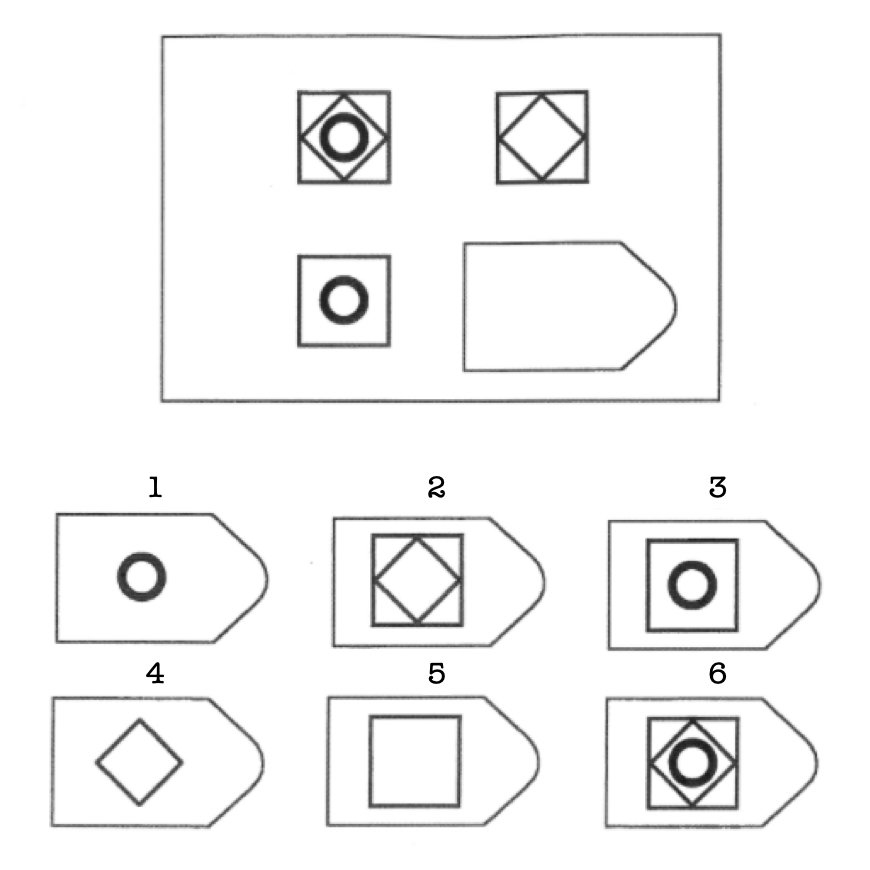
\includegraphics[scale=0.2]{Ravens Survey.jpg}
\end{figure}

\noindent First, notice a square in the upper left, the upper right, and the lower left. Also, notice that the circle is eliminated when one moves from the upper left to the upper right. Finally, the rhombus is eliminated when moving from the upper left to the lower left. Therefore, the correct piece should eliminate the circle and the rhombus, leaving only a square. So, the correct answer is piece 5. \\

\noindent To give your answer to each image, you must choose the correct option and then continue to the next screen. After giving your answer you cannot go back. \\

\noindent You will have 5 minutes to complete the test, which consists of 18 images to solve. The percentage of correct answers will determine your chances of winning one of the 100.000 pesos bonuses if you are chosen for the drawing. \\

\noindent\rule{\textwidth}{0.4pt}\\

\noindent Are you ready? \\
 
\noindent Your 5 minutes will start as soon as you move to the next screen. \\

\noindent\rule{\textwidth}{0.4pt}\\

\noindent \textbf{Problem 1}\\

\noindent [screenshot of Raven's matrix] \\

\noindent [After participants submit an answer, a new matrix appears on the screen. The sequence of matrices is the same for all participants. Participants cannot return to a previous screen. Participants do not have to provide answers for all 18 matrices.] \\

\noindent\rule{\textwidth}{0.4pt}\\

\noindent You have finished the test. You can proceed to the next screen. \\

\noindent\rule{\textwidth}{0.4pt}\\

\noindent \textbf{How did you do on the test?} \\

\noindent If we randomly choose 10 participants from this classroom, how many people do you think solved fewer correct problems than you?\\

\noindent [Slider from 0 to 10]\\

\noindent\rule{\textwidth}{0.4pt}\\

\noindent \textbf{Test - Emotions} \\
 
\noindent In this test, you will see a series of photographs. Below is an example of the pictures you will see. In each picture, you will see the eyes of a person. Below the picture, you will see four possible emotions that this person is feeling. Your task is to choose which of the four emotions correctly describes what the person is feeling. For each picture, there is only one emotion. Look at the following example: \\

\begin{figure}[htbp]
  \centering
  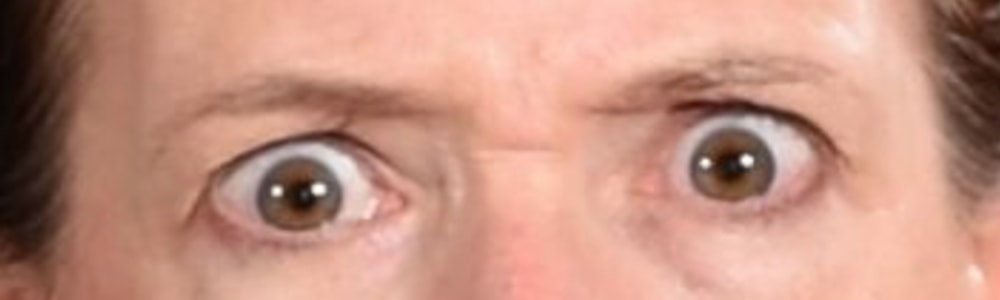
\includegraphics[scale=0.2]{3Aghast-J.jpg}
\end{figure}

\noindent [Happy, Disappointed, Shocked, Worried] \\

\noindent In this case, the correct answer is: Shocked. \\

\noindent To give your answer to each picture, you must choose the correct option and then continue to the next screen. After giving your answer you will not be able to go back. \\

\noindent You will have 5 minutes to complete the test, which consists of 36 photographs to solve. The percentage of correct answers you get will determine your chances of winning one of the 100.000 pesos bonuses if you are chosen for the drawing. \\

\noindent\rule{\textwidth}{0.4pt}\\

\noindent Are you ready? \\
 
\noindent Your 5 minutes will start as soon as you move to the next screen. \\

\noindent\rule{\textwidth}{0.4pt}\\

\noindent \textbf{Photograph 1: Choose the word that best describes the photograph} \\

\noindent [photo from Multiracial Reading the Mind in the Eyes Test] \\

\noindent [After participants submit an answer, a new photo appears on the screen. The sequence of photos is the same for all participants. Participants cannot return to a previous screen. Participants do not have to provide answers for all 36 photos.] \\

\noindent\rule{\textwidth}{0.4pt}\\

\noindent You have finished the test. You can proceed to the next screen. \\

\noindent\rule{\textwidth}{0.4pt}\\

\noindent \textbf{How did you do on the test?} \\

\noindent If we randomly choose 10 participants from this classroom, how many people do you think solved fewer correct photographs than you?\\

\noindent [Slider from 0 to 10]\\

\noindent\rule{\textwidth}{0.4pt}\\

\noindent \textbf{Part 2} \\
 
\noindent At the beginning of this study, all participants took two tests, one on cognitive ability and one on emotions. In this part, we will ask you to recommend the people who in your opinion will score the best on each test. \\

\noindent You may recommend 3 people per test, but you may not recommend yourself. \\

\noindent We will allocate up to [classroom-specific number equal to 40\% of class size] bonuses of 100.000 pesos for Part 2. The steps for allocating bonuses are explained below. \\

\noindent\rule{\textwidth}{0.4pt}\\

\noindent [random assignment to either quota or baseline condition] \\

\noindent [classroom-specific illustrations explaining the incentive structure depending on assignment to either baseline or quota conditions] \\

\noindent\rule{\textwidth}{0.4pt}\\

\noindent [random assignment to either cognitive or social skills referral task] \\

\noindent \textbf{Recommendation - Cognitive Skill}\\

\noindent All participants took a test to identify the missing pattern in each image, as in the example below. This test is used to measure general intelligence.\\

\begin{figure}[htbp]
  \centering
  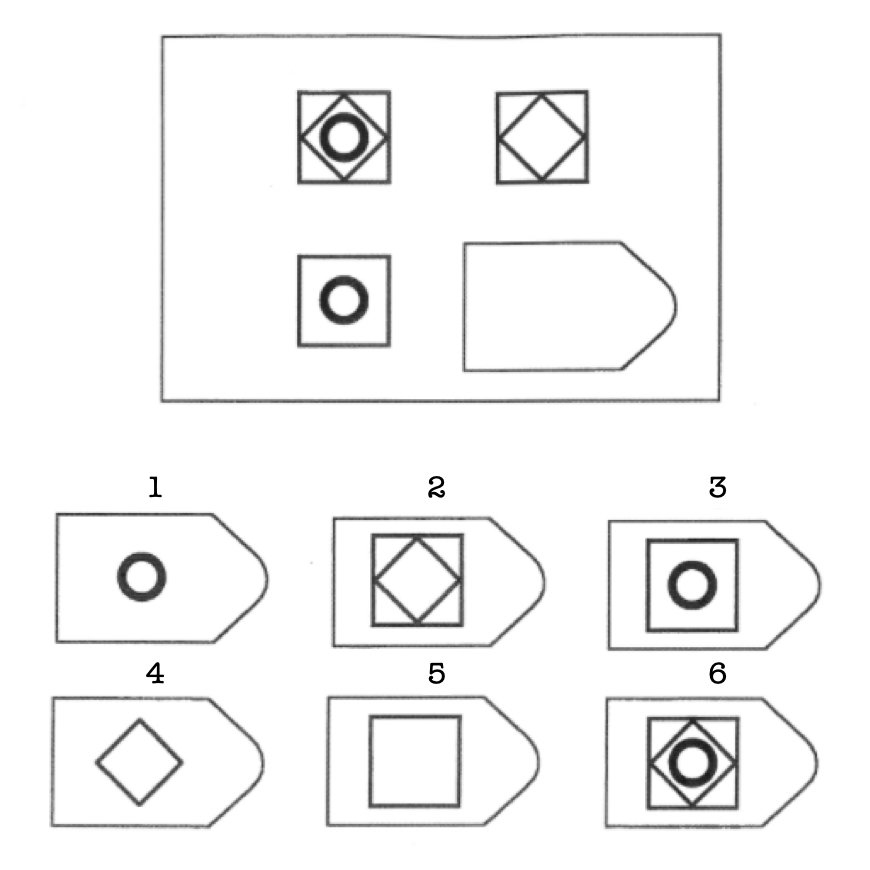
\includegraphics[scale=0.2]{Ravens Survey.jpg}
\end{figure}

\noindent Next, we will present you with a list of the names of all the students in this room. We will ask you to recommend the three people you think will score the highest on the general intelligence test. \\

\noindent If you are chosen by the computer, each of your recommendations in the top 3 increases your chances of winning one of the 100.000 pesos bonuses. \\

\noindent\rule{\textwidth}{0.4pt}\\

\noindent Select the students in this classroom who you consider to have the highest scores on the general intelligence test. (Select 3 students) \\

\noindent [Classroom-specific list of all classmate names visible on one screen. Participants have to pick 3 classmates to continue. Picking their own name invalidates their choices.]\\

\noindent\rule{\textwidth}{0.4pt}\\

\noindent \textbf{Recommendation - Emotions} \\

\noindent All participants took a test where they had to identify the emotion that best described the expression of each image as in the example below. This test is used to measure social skills. \\

\begin{figure}[htbp]
  \centering
  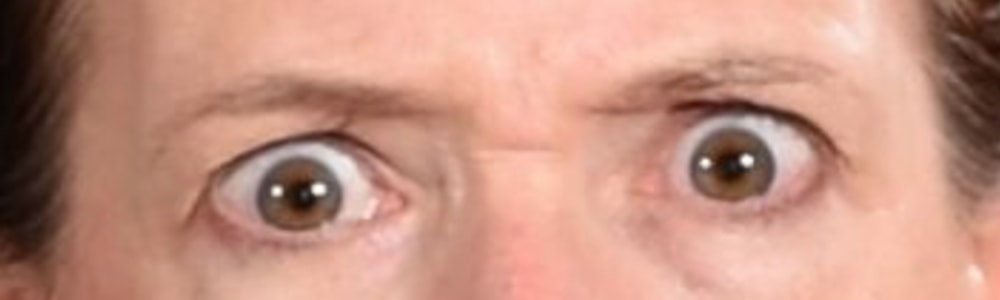
\includegraphics[scale=0.2]{3Aghast-J.jpg}
\end{figure}

\noindent Next, we will present you with a list of the names of all the students in this room. We will ask you to recommend 3 people you think will score the highest on the social skills test. \\

\noindent If you are chosen by the computer, each of your recommendations in the top 3 increases your chances of winning one of the 100.000 pesos bonuses. \\

\noindent\rule{\textwidth}{0.4pt}\\

\noindent Select the students in this classroom who you consider to have the highest scores on the social skills test. (Select 3 students) \\

\noindent [Classroom-specific list of all the names visible on one screen. Participants have to pick 3 classmates to continue. Picking their own name invalidates their choices.]\\

\noindent\rule{\textwidth}{0.4pt}\\

\noindent\textbf{Part 3: Recommendation - Random draw}

\noindent In this part, the computer will randomly choose three students who belong to strata 1, 2, or 3. We will ask you to nominate three people you think the computer will choose. \\

\noindent We will allocate up to [classroom-specific number equal to 20\% of class size] bonuses of 100.000 pesos for Part 3. The steps for allocating the bonuses are explained below. \\

\noindent\rule{\textwidth}{0.4pt}\\

\noindent [classroom-specific illustrations explaining the incentive structure] \\

\noindent\rule{\textwidth}{0.4pt}\\

\noindent Select the students in this classroom who belong to strata 1, 2, or 3, who you think will be randomly selected by the computer (Select 3 students). \\

\noindent [Classroom-specific list of all the names visible on one screen. Participants have to pick 3 classmates to continue. Picking their own name invalidates their choices.]\\

\noindent\rule{\textwidth}{0.4pt}\\

\noindent \textbf{Part 4}

\noindent Do you want to know your scores on the general intelligence test and the social skills test? We can analyze the data and give you a report that explains your strengths in these two areas. Also, what do these strengths mean, and how can you leverage them for your personal and professional development? \\

\noindent If you want to receive your skills report, we need to contact you again. We also want to be able to invite you to new studies where you can participate for more bonus money. Please indicate if you agree to be contacted again. \\

\noindent [I can be contacted for new studies and to send me my report. I can be contacted to send my report, but not for new studies.  No, I do not want to be contacted again.]

\noindent\rule{\textwidth}{0.4pt}\\

\noindent [if participant gives consent to be contacted again] \\

\noindent Please enter your contact email: \\

\noindent [student email]\\

\end{document}
